%
% These examples are based on the package documentation:
% http://www.ctan.org/tex-archive/macros/latex/contrib/minted
%
\documentclass{article}
\usepackage{graphicx}
\usepackage[T1]{fontenc}
\usepackage[utf8]{inputenc}
\usepackage{lmodern}

\usepackage{minted}

\begin{document}

\title{Wireshark Packet Capture}
\author{Amrith M}
\maketitle

\section{About Wireshark}
Wireshark is a free and open source packet analyzer. It is used for network troubleshooting, analysis, software and communications protocol development, and education. Originally named Ethereal, the project was renamed Wireshark in May 2006 due to trademark issues.[5]

Wireshark is cross-platform, using the Qt widget toolkit in current releases to implement its user interface, and using pcap to capture packets; it runs on Linux, macOS, BSD, Solaris, some other Unix-like operating systems, and Microsoft Windows. There is also a terminal-based (non-GUI) version called TShark. Wireshark, and the other programs distributed with it such as TShark, are free software, released under the terms of the GNU General Public License.

\section{TCP Packet Capture}
TCP Packets are captured and 3-way handshake is observed. (figure below)
\begin{figure}
\centering
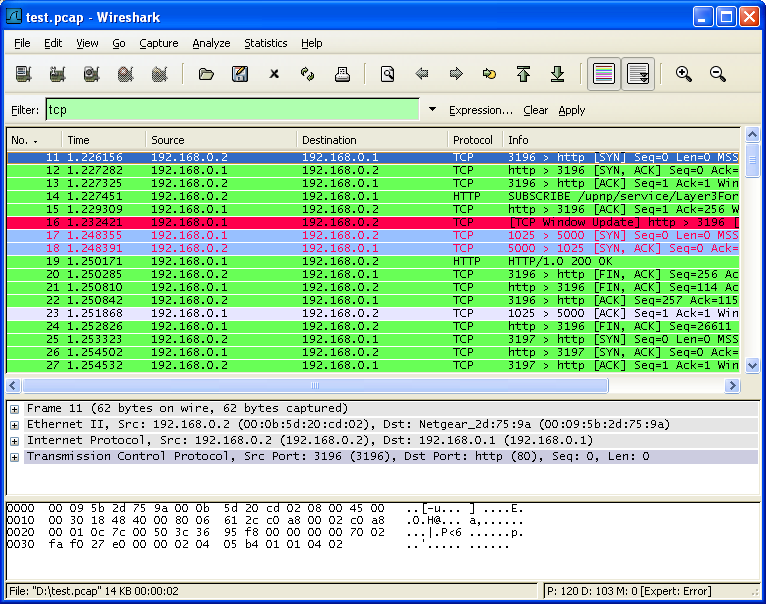
\includegraphics[width=\textwidth,height=\textheight,keepaspectratio]{TCP.png}
\end{figure}

\section{UDP Packet Capture}
UDP packets are captured and sending datagrams in a connectionless service is observed. (figure below)
\begin{figure}
\centering
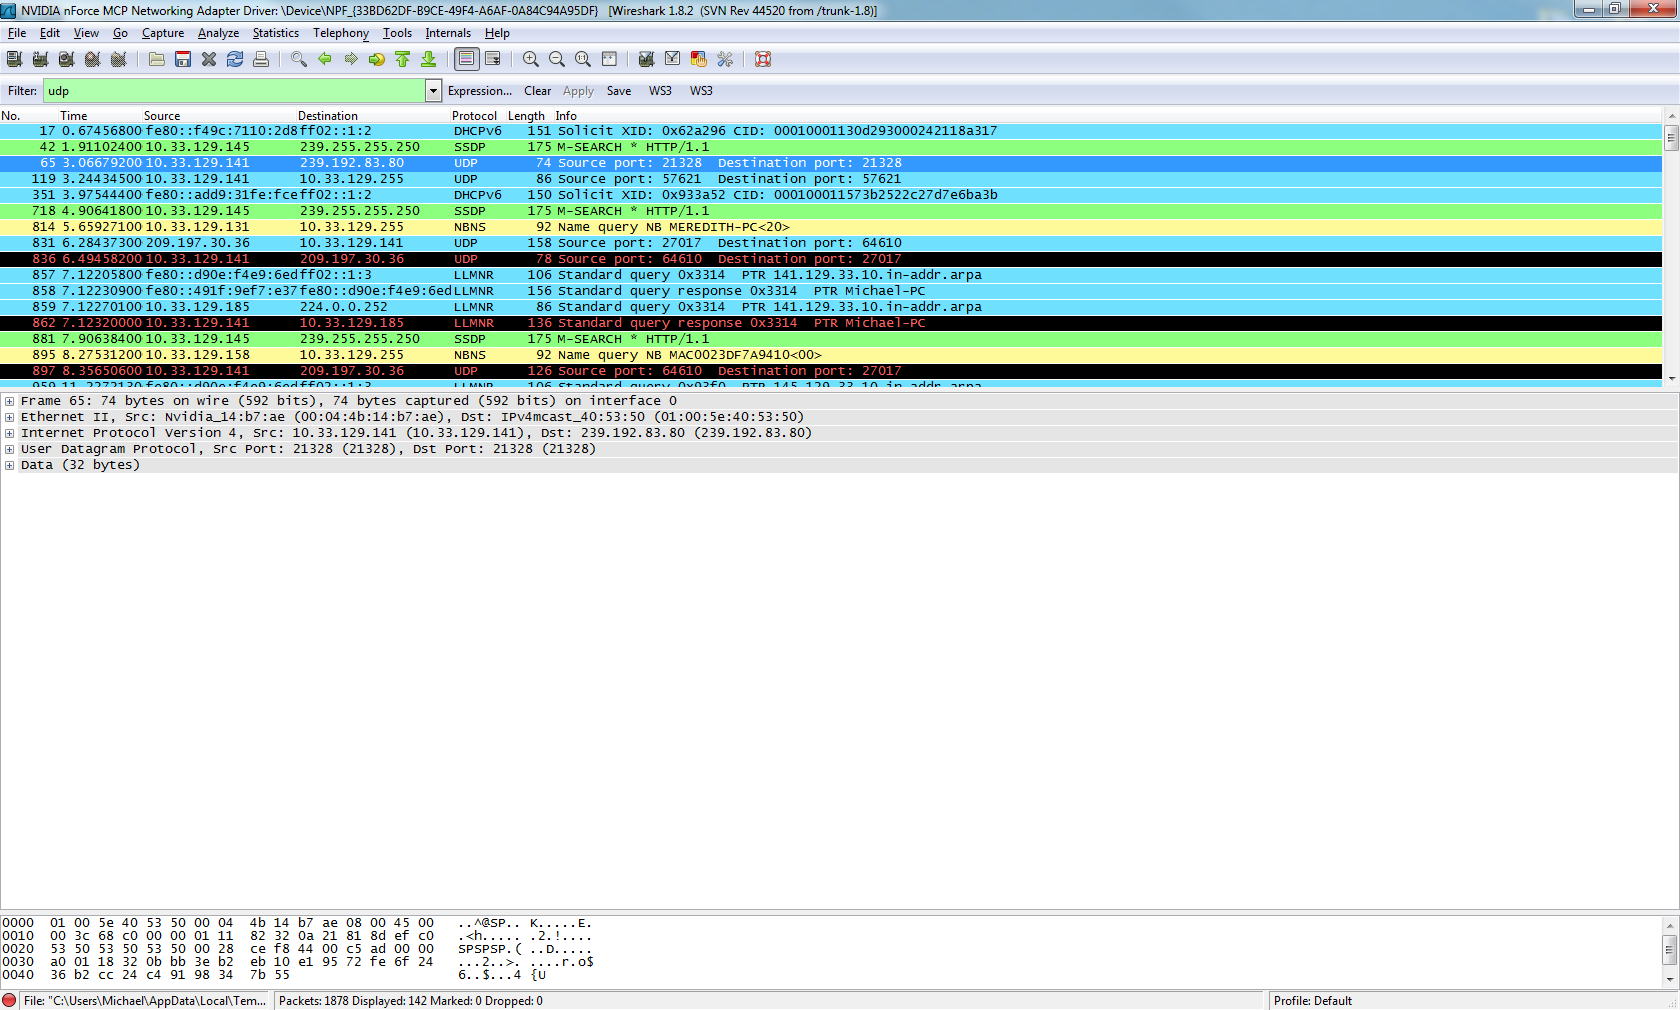
\includegraphics[width=\textwidth,height=\textheight,keepaspectratio]{UDP.png}
\end{figure}
\end{document}